\documentclass[11pt]{article}
\usepackage{amsmath,amssymb}
\usepackage{tikz}
\usetikzlibrary{decorations.pathreplacing,calc}
\usepackage[margin=0.8in]{geometry}

%% Ring colours (6 rings for max entry 6)
\definecolor{ring1}{RGB}{220,235,255}
\definecolor{ring2}{RGB}{170,200,255}
\definecolor{ring3}{RGB}{120,165,255}
\definecolor{ring4}{RGB}{80,130,220}
\definecolor{ring5}{RGB}{50,95,190}
\definecolor{ring6}{RGB}{30,60,160}

\title{Cylindric Plane Partition\\[4pt]
  $\mathfrak{c} = \bigl((3,2,2),\;(4,3,2,1),\;(4,3,2),\;(6,4,3,2),\;(5,3,2),\;(3,2,2)\bigr)$\\[4pt]
  Profile $\pi = 10100$}
\author{Generated from thesis examples}
\date{}

\begin{document}
\maketitle

%% ============================================================
\section{Labelled cylindric diagram (numbers on faces)}
%% ============================================================

The fundamental domain of the cylindric diagram with profile $\pi = 10100$.
Each entry gives the height of the cube stack at that position.
The NW--SE diagonals (from right to left) read off
$\mu^0 = (3,2,2)$, $\mu^1 = (4,3,2,1)$, $\mu^2 = (4,3,2)$,
$\mu^3 = (6,4,3,2)$, $\mu^4 = (5,3,2)$.

\bigskip
\begin{center}
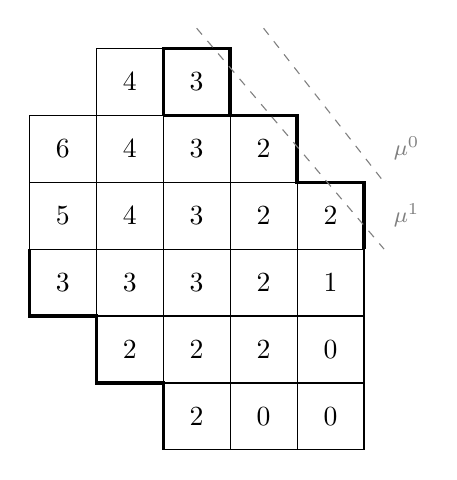
\begin{tikzpicture}[scale=0.85]
  % Helper: draw a cell at (col, row) in English convention (row 0 = top)
  % with label text. Thick edges on the staircase boundary.
  \newcommand{\cell}[3]{% col, row, label
    \fill[white] (#1, -#2) rectangle ++(1,-1);
    \draw (#1, -#2) rectangle ++(1,-1);
    \node at (#1+0.5, -#2-0.5) {$#3$};
  }

  % Row 0 (top): cols 1-2, entries 4, 3
  \cell{1}{0}{4}  \cell{2}{0}{3}
  % Row 1: cols 0-3, entries 6, 4, 3, 2
  \cell{0}{1}{6}  \cell{1}{1}{4}  \cell{2}{1}{3}  \cell{3}{1}{2}
  % Row 2: cols 0-4, entries 5, 4, 3, 2, 2
  \cell{0}{2}{5}  \cell{1}{2}{4}  \cell{2}{2}{3}  \cell{3}{2}{2}  \cell{4}{2}{2}
  % Row 3: cols 0-4, entries 3, 3, 3, 2, 1
  \cell{0}{3}{3}  \cell{1}{3}{3}  \cell{2}{3}{3}  \cell{3}{3}{2}  \cell{4}{3}{1}
  % Row 4: cols 1-4, entries 2, 2, 2, 0
  \cell{1}{4}{2}  \cell{2}{4}{2}  \cell{3}{4}{2}  \cell{4}{4}{0}
  % Row 5: cols 2-4, entries 2, 0, 0
  \cell{2}{5}{2}  \cell{3}{5}{0}  \cell{4}{5}{0}

  %% Upper-right staircase boundary (thick)
  \draw[very thick] (2,-1) -- (3,-1) -- (3,0) -- (2,0) -- (2,-1);
  \draw[very thick] (3,0) -- (3,-1) -- (4,-1) -- (4,-2) -- (5,-2) -- (5,-3);

  %% Lower-left staircase boundary (thick)
  \draw[very thick] (0,-3) -- (0,-4) -- (1,-4) -- (1,-5) -- (2,-5) -- (2,-6);

  %% Diagonal labels
  \draw[gray, dashed, thin] (3.5, 0.3) -- (5.3, -2.0);
  \node[gray, right] at (5.3,-1.5) {\footnotesize $\mu^0$};
  \draw[gray, dashed, thin] (2.5, 0.3) -- (5.3, -3.0);
  \node[gray, right] at (5.3,-2.5) {\footnotesize $\mu^1$};
\end{tikzpicture}
\end{center}


%% ============================================================
\section{Ring colouring (PEEL)}
%% ============================================================

Each cell in column~$j$ of a Young diagram belongs to \textbf{ring~$j$}.
The growth diagram has $\max(\mathfrak{c}) = 6$ concentric rings.
Peeling ring~$k$ demotes all parts equal to~$k$ by one.

\bigskip
\begin{center}
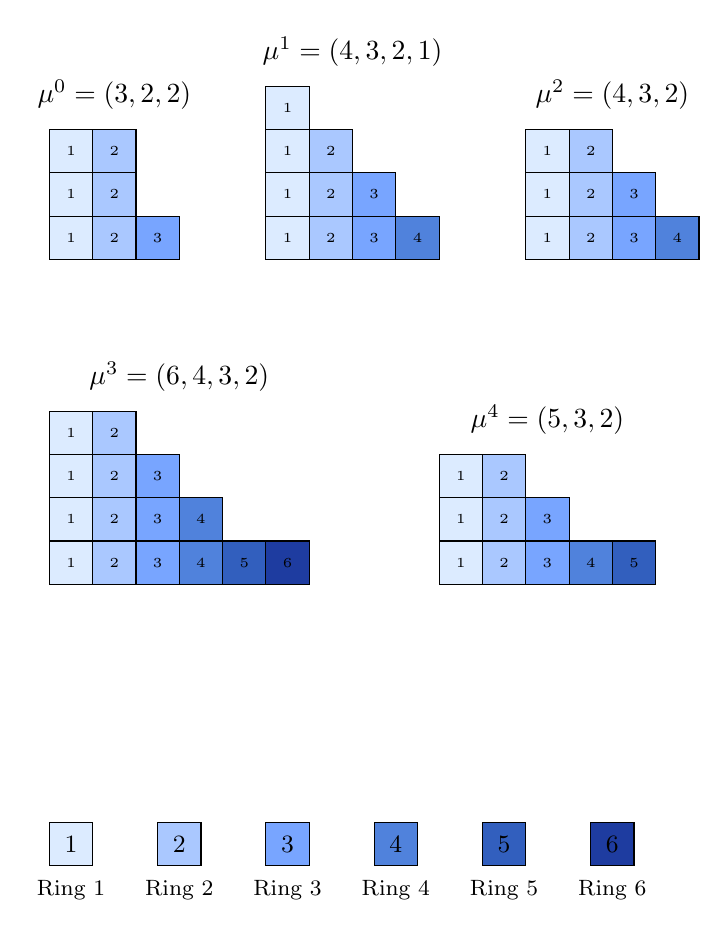
\begin{tikzpicture}[scale=0.55]
  % Macro: draw partition in French convention (row 1 = bottom)
  % Arguments: xshift, partition parts as comma list, title
  \newcommand{\ringcell}[4]{% x, y (from bottom), col (1-indexed), value
    \pgfmathtruncatemacro{\ringnum}{#3}
    \ifcase\ringnum\or
      \fill[ring1] (#1,#2) rectangle ++(1,1);\or
      \fill[ring2] (#1,#2) rectangle ++(1,1);\or
      \fill[ring3] (#1,#2) rectangle ++(1,1);\or
      \fill[ring4] (#1,#2) rectangle ++(1,1);\or
      \fill[ring5] (#1,#2) rectangle ++(1,1);\or
      \fill[ring6] (#1,#2) rectangle ++(1,1);\fi
    \draw (#1,#2) rectangle ++(1,1);
    \node[font=\tiny] at (#1+0.5,#2+0.5) {#3};
  }

  %% mu^0 = (3,2,2) -- French convention: bottom row = longest
  \begin{scope}[xshift=0cm]
    \node at (1.5, 3.8) {$\mu^0 = (3,2,2)$};
    % Row 1 (bottom): 3 cells
    \ringcell{0}{0}{1}{} \ringcell{1}{0}{2}{} \ringcell{2}{0}{3}{}
    % Row 2: 2 cells
    \ringcell{0}{1}{1}{} \ringcell{1}{1}{2}{}
    % Row 3: 2 cells
    \ringcell{0}{2}{1}{} \ringcell{1}{2}{2}{}
  \end{scope}

  %% mu^1 = (4,3,2,1)
  \begin{scope}[xshift=5cm]
    \node at (2, 4.8) {$\mu^1 = (4,3,2,1)$};
    % Row 1: 4 cells
    \ringcell{0}{0}{1}{} \ringcell{1}{0}{2}{} \ringcell{2}{0}{3}{} \ringcell{3}{0}{4}{}
    % Row 2: 3 cells
    \ringcell{0}{1}{1}{} \ringcell{1}{1}{2}{} \ringcell{2}{1}{3}{}
    % Row 3: 2 cells
    \ringcell{0}{2}{1}{} \ringcell{1}{2}{2}{}
    % Row 4: 1 cell
    \ringcell{0}{3}{1}{}
  \end{scope}

  %% mu^2 = (4,3,2)
  \begin{scope}[xshift=11cm]
    \node at (2, 3.8) {$\mu^2 = (4,3,2)$};
    % Row 1: 4 cells
    \ringcell{0}{0}{1}{} \ringcell{1}{0}{2}{} \ringcell{2}{0}{3}{} \ringcell{3}{0}{4}{}
    % Row 2: 3 cells
    \ringcell{0}{1}{1}{} \ringcell{1}{1}{2}{} \ringcell{2}{1}{3}{}
    % Row 3: 2 cells
    \ringcell{0}{2}{1}{} \ringcell{1}{2}{2}{}
  \end{scope}

  %% mu^3 = (6,4,3,2)
  \begin{scope}[xshift=0cm, yshift=-7.5cm]
    \node at (3, 4.8) {$\mu^3 = (6,4,3,2)$};
    % Row 1: 6 cells
    \ringcell{0}{0}{1}{} \ringcell{1}{0}{2}{} \ringcell{2}{0}{3}{}
    \ringcell{3}{0}{4}{} \ringcell{4}{0}{5}{} \ringcell{5}{0}{6}{}
    % Row 2: 4 cells
    \ringcell{0}{1}{1}{} \ringcell{1}{1}{2}{} \ringcell{2}{1}{3}{} \ringcell{3}{1}{4}{}
    % Row 3: 3 cells
    \ringcell{0}{2}{1}{} \ringcell{1}{2}{2}{} \ringcell{2}{2}{3}{}
    % Row 4: 2 cells
    \ringcell{0}{3}{1}{} \ringcell{1}{3}{2}{}
  \end{scope}

  %% mu^4 = (5,3,2)
  \begin{scope}[xshift=9cm, yshift=-7.5cm]
    \node at (2.5, 3.8) {$\mu^4 = (5,3,2)$};
    % Row 1: 5 cells
    \ringcell{0}{0}{1}{} \ringcell{1}{0}{2}{} \ringcell{2}{0}{3}{}
    \ringcell{3}{0}{4}{} \ringcell{4}{0}{5}{}
    % Row 2: 3 cells
    \ringcell{0}{1}{1}{} \ringcell{1}{1}{2}{} \ringcell{2}{1}{3}{}
    % Row 3: 2 cells
    \ringcell{0}{2}{1}{} \ringcell{1}{2}{2}{}
  \end{scope}

  %% Legend
  \begin{scope}[xshift=0cm, yshift=-14cm]
    \foreach \r/\c/\lab in {1/ring1/1, 2/ring2/2, 3/ring3/3, 4/ring4/4, 5/ring5/5, 6/ring6/6} {
      \pgfmathsetmacro{\xpos}{(\r-1)*2.5}
      \fill[\c] (\xpos,0) rectangle ++(1,1);
      \draw (\xpos,0) rectangle ++(1,1);
      \node at (\xpos+0.5, 0.5) {\small \lab};
      \node[below] at (\xpos+0.5, -0.1) {\footnotesize Ring \lab};
    }
  \end{scope}
\end{tikzpicture}
\end{center}


%% ============================================================
\section{Growth diagram with ALCD}
%% ============================================================

The cylindric growth diagram with profile $\pi = 00101$
(rotation of $10100$).
Vertex labels are partitions; face labels are the ALCD entries.
Base partition $\gamma = (3,2)$.

\bigskip
\begin{center}
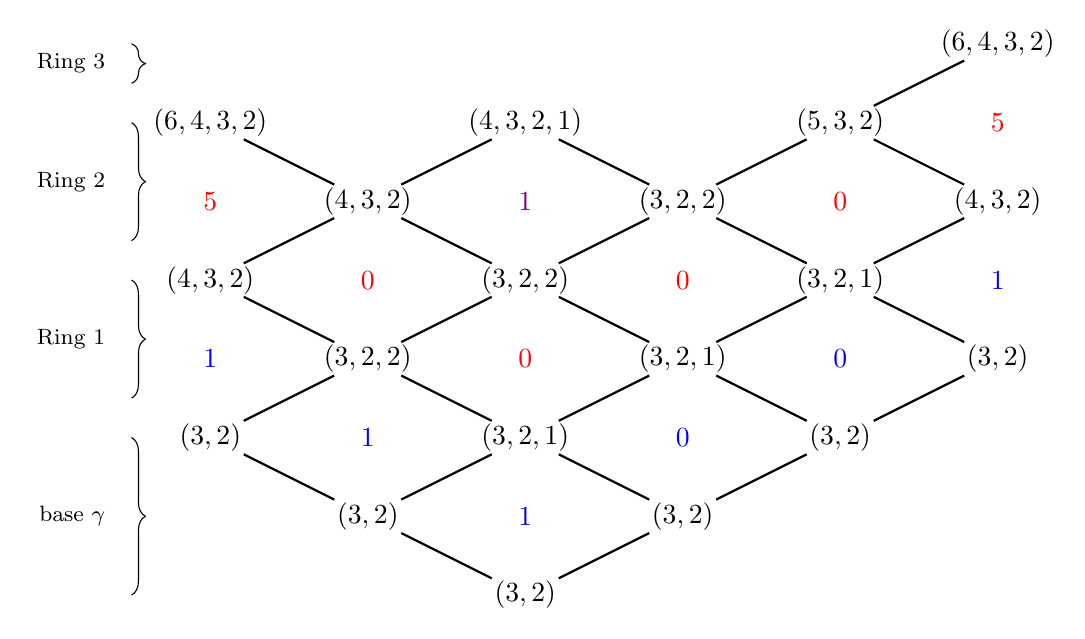
\begin{tikzpicture}[scale=1]
  % Level 0 (base): all vertices = (3,2)
  \path (-4,2) node[inner sep=0.3mm](A0){$(3,2)$};
  \path (-2,1) node[inner sep=0.3mm](B0){$(3,2)$};
  \path (0,0)  node[inner sep=0.3mm](C0){$(3,2)$};
  \path (2,1)  node[inner sep=0.3mm](D0){$(3,2)$};
  \path (4,2)  node[inner sep=0.3mm](E0){$(3,2)$};
  \path (6,3)  node[inner sep=0.3mm](F0){$(3,2)$};

  % Level 1
  \path (-4,4) node[inner sep=0.3mm](A1){$(4,3,2)$};
  \path (-2,3) node[inner sep=0.3mm](B1){$(3,2,2)$};
  \path (0,2)  node[inner sep=0.3mm](C1){$(3,2,1)$};
  \path (2,3)  node[inner sep=0.3mm](D1){$(3,2,1)$};
  \path (4,4)  node[inner sep=0.3mm](E1){$(3,2,1)$};
  \path (6,5)  node[inner sep=0.3mm](F1){$(4,3,2)$};

  % Level 2
  \path (-4,6) node[inner sep=0.3mm](A2){$(6,4,3,2)$};
  \path (-2,5) node[inner sep=0.3mm](B2){$(4,3,2)$};
  \path (0,4)  node[inner sep=0.3mm](C2){$(3,2,2)$};
  \path (2,5)  node[inner sep=0.3mm](D2){$(3,2,2)$};
  \path (4,6)  node[inner sep=0.3mm](E2){$(5,3,2)$};
  \path (6,7)  node[inner sep=0.3mm](F2){$(6,4,3,2)$};

  % Level 3 (peak)
  \path (0,6) node[inner sep=0.3mm](C3){$(4,3,2,1)$};

  %% Horizontal edges (paths at each level)
  \draw[thick] (A0) -- (B0) -- (C0) -- (D0) -- (E0) -- (F0);
  \draw[thick] (A1) -- (B1) -- (C1) -- (D1) -- (E1) -- (F1);
  \draw[thick] (A2) -- (B2) -- (C2) -- (D2) -- (E2) -- (F2);

  %% Diagonal edges (NW direction, profile 1-steps)
  \draw[thick] (A1) -- (B2) -- (C3);
  %% Diagonal edges (SW direction, profile 0-steps)
  \draw[thick] (A0) -- (B1) -- (C2);
  \draw[thick] (B0) -- (C1);
  \draw[thick] (D0) -- (C1);
  \draw[thick] (E0) -- (D1) -- (C2);
  \draw[thick] (F0) -- (E1) -- (D2) -- (C3);
  \draw[thick] (F1) -- (E2);

  %% Face labels: Ring 1 (between levels 0 and 1)
  \node[blue] at (-4,3) {$1$};
  \node[blue] at (-2,2) {$1$};
  \node[blue] at (0,1)  {$1$};
  \node[blue] at (2,2)  {$0$};
  \node[blue] at (4,3)  {$0$};
  \node[blue] at (6,4)  {$1$};

  %% Face labels: Ring 2 (between levels 1 and 2)
  \node[red] at (-4,5) {$5$};
  \node[red] at (-2,4) {$0$};
  \node[red] at (0,3)  {$0$};
  \node[red] at (2,4)  {$0$};
  \node[red] at (4,5)  {$0$};
  \node[red] at (6,6)  {$5$};

  %% Face label: Ring 3 (between levels 2 and 3)
  \node[violet] at (0,5) {$1$};

  %% Boundary annotation
  \draw[decorate, decoration={brace, amplitude=5pt, mirror}]
    (-5, 0) -- (-5, 2) node[midway, left=6pt] {\footnotesize base $\gamma$};
  \draw[decorate, decoration={brace, amplitude=5pt, mirror}]
    (-5, 2.5) -- (-5, 4) node[midway, left=6pt] {\footnotesize Ring 1};
  \draw[decorate, decoration={brace, amplitude=5pt, mirror}]
    (-5, 4.5) -- (-5, 6) node[midway, left=6pt] {\footnotesize Ring 2};
  \draw[decorate, decoration={brace, amplitude=5pt, mirror}]
    (-5, 6.5) -- (-5, 7) node[midway, left=6pt] {\footnotesize Ring 3};
\end{tikzpicture}
\end{center}


%% ============================================================
\section{The ALCD (face labels only)}
%% ============================================================

Forgetting the vertex labels and retaining only the face labels
gives the arbitrarily labelled cylindric diagram.
Depth~$= 3$, weight $= 1 \times 1 + 5 \times 1 + 1 \times 4 + 1 \times 7 + 1 \times 9 = 26$.

\bigskip
\begin{center}
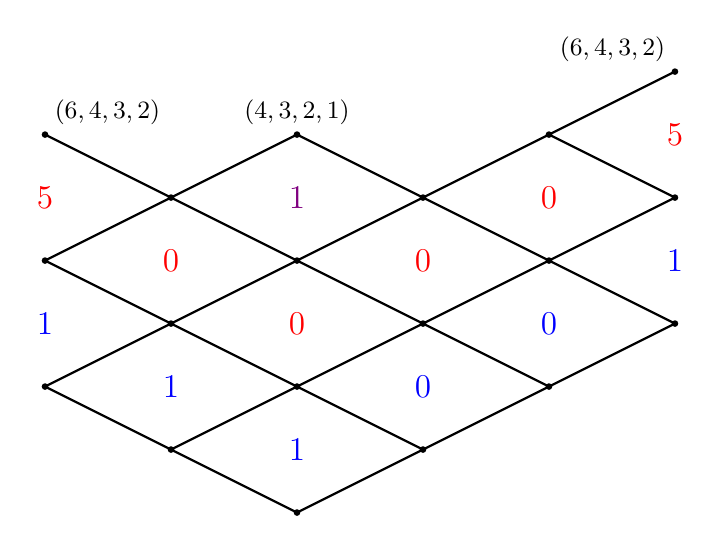
\begin{tikzpicture}[scale=0.8]
  % Same graph structure, no vertex labels, only face labels
  \foreach \name/\x/\y in {A0/-4/2, B0/-2/1, C0/0/0, D0/2/1, E0/4/2, F0/6/3,
                            A1/-4/4, B1/-2/3, C1/0/2, D1/2/3, E1/4/4, F1/6/5,
                            A2/-4/6, B2/-2/5, C2/0/4, D2/2/5, E2/4/6, F2/6/7,
                            C3/0/6} {
    \coordinate (\name) at (\x, \y);
    \fill (\x,\y) circle (1.5pt);
  }

  \draw[thick] (A0) -- (B0) -- (C0) -- (D0) -- (E0) -- (F0);
  \draw[thick] (A1) -- (B1) -- (C1) -- (D1) -- (E1) -- (F1);
  \draw[thick] (A2) -- (B2) -- (C2) -- (D2) -- (E2) -- (F2);
  \draw[thick] (A1) -- (B2) -- (C3);
  \draw[thick] (A0) -- (B1) -- (C2);
  \draw[thick] (B0) -- (C1);
  \draw[thick] (D0) -- (C1);
  \draw[thick] (E0) -- (D1) -- (C2);
  \draw[thick] (F0) -- (E1) -- (D2) -- (C3);
  \draw[thick] (F1) -- (E2);

  %% Face labels
  \node[blue, font=\large] at (-4,3) {$1$};
  \node[blue, font=\large] at (-2,2) {$1$};
  \node[blue, font=\large] at (0,1)  {$1$};
  \node[blue, font=\large] at (2,2)  {$0$};
  \node[blue, font=\large] at (4,3)  {$0$};
  \node[blue, font=\large] at (6,4)  {$1$};

  \node[red, font=\large] at (-4,5) {$5$};
  \node[red, font=\large] at (-2,4) {$0$};
  \node[red, font=\large] at (0,3)  {$0$};
  \node[red, font=\large] at (2,4)  {$0$};
  \node[red, font=\large] at (4,5)  {$0$};
  \node[red, font=\large] at (6,6)  {$5$};

  \node[violet, font=\large] at (0,5) {$1$};

  %% Upper boundary partition labels
  \node[above right, font=\small] at (A2) {$(6,4,3,2)$};
  \node[above, font=\small] at (C3) {$(4,3,2,1)$};
  \node[above left, font=\small] at (F2) {$(6,4,3,2)$};
\end{tikzpicture}
\end{center}

The ALCD in tableau form (on the cylindric diagram fundamental domain):
\[
\begin{array}{ccccc}
  & 1 & 0 \\
5 & 0 & 0 & 0 \\
0 & 1 & 1 & 1 & 0 \\
0 & 0 & 0 & 0 & 0 \\
  & 0 & 0 & 0 & 0 \\
  &   & 0 & 0 & 0
\end{array}
\]


%% ============================================================
\section{Non-intersecting lattice paths (page 81)}
%% ============================================================

The CPP corresponds to a family of 7 non-intersecting lattice paths
on the cylinder of period $T = 5$.
Black vertices are occupied (path passes through);
white vertices are unoccupied.

\bigskip
\begin{center}
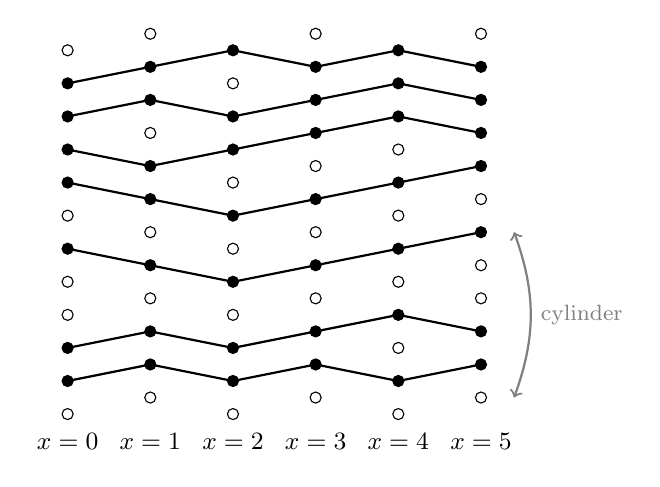
\begin{tikzpicture}[scale=0.42,
    bvert/.style={circle, fill=black, inner sep=0, minimum size=4pt},
    wvert/.style={circle, draw=black, fill=white, inner sep=0, minimum size=4pt}
  ]

  %% Path data: 7 paths, each with y-values at x=0..5
  %% p1: (1,0,1,0,1), y0=2  -> y: 2,3,2,3,2,3
  %% p2: (1,0,1,1,0), y0=4  -> y: 4,5,4,5,6,5
  %% p3: (0,0,1,1,1), y0=10 -> y: 10,9,8,9,10,11
  %% p4: (0,0,1,1,1), y0=14 -> y: 14,13,12,13,14,15
  %% p5: (0,1,1,1,0), y0=16 -> y: 16,15,16,17,18,17
  %% p6: (1,0,1,1,0), y0=18 -> y: 18,19,18,19,20,19
  %% p7: (1,1,0,1,0), y0=20 -> y: 20,21,22,21,22,21

  % Collect all occupied y-values per column
  % x=0 (even): 2,4,10,14,16,18,20
  % x=1 (odd):  3,5,9,13,15,19,21
  % x=2 (even): 2,4,8,12,16,18,22
  % x=3 (odd):  3,5,9,13,17,19,21
  % x=4 (even): 2,6,10,14,18,20,22
  % x=5 (odd):  3,5,11,15,17,19,21

  % Draw all vertices in the triangular lattice (x,y) with x+y even
  \foreach \x in {0,...,5} {
    \pgfmathtruncatemacro{\parity}{mod(\x,2)}
    \ifnum\parity=0
      \foreach \y in {0,2,...,22} {
        \node[wvert] (v\x-\y) at (\x*2.5, \y*0.5) {};
      }
    \else
      \foreach \y in {1,3,...,23} {
        \node[wvert] (v\x-\y) at (\x*2.5, \y*0.5) {};
      }
    \fi
  }

  % Mark occupied vertices black
  % x=0: 2,4,10,14,16,18,20
  \foreach \y in {2,4,10,14,16,18,20} {
    \node[bvert] at (0*2.5, \y*0.5) {};
  }
  % x=1: 3,5,9,13,15,19,21
  \foreach \y in {3,5,9,13,15,19,21} {
    \node[bvert] at (1*2.5, \y*0.5) {};
  }
  % x=2: 2,4,8,12,16,18,22
  \foreach \y in {2,4,8,12,16,18,22} {
    \node[bvert] at (2*2.5, \y*0.5) {};
  }
  % x=3: 3,5,9,13,17,19,21
  \foreach \y in {3,5,9,13,17,19,21} {
    \node[bvert] at (3*2.5, \y*0.5) {};
  }
  % x=4: 2,6,10,14,18,20,22
  \foreach \y in {2,6,10,14,18,20,22} {
    \node[bvert] at (4*2.5, \y*0.5) {};
  }
  % x=5: 3,5,11,15,17,19,21
  \foreach \y in {3,5,11,15,17,19,21} {
    \node[bvert] at (5*2.5, \y*0.5) {};
  }

  % Draw path edges (thick lines connecting consecutive occupied vertices)
  % p1: 2->3->2->3->2->3
  \draw[thick] (0*2.5,2*0.5) -- (1*2.5,3*0.5) -- (2*2.5,2*0.5)
    -- (3*2.5,3*0.5) -- (4*2.5,2*0.5) -- (5*2.5,3*0.5);
  % p2: 4->5->4->5->6->5
  \draw[thick] (0*2.5,4*0.5) -- (1*2.5,5*0.5) -- (2*2.5,4*0.5)
    -- (3*2.5,5*0.5) -- (4*2.5,6*0.5) -- (5*2.5,5*0.5);
  % p3: 10->9->8->9->10->11
  \draw[thick] (0*2.5,10*0.5) -- (1*2.5,9*0.5) -- (2*2.5,8*0.5)
    -- (3*2.5,9*0.5) -- (4*2.5,10*0.5) -- (5*2.5,11*0.5);
  % p4: 14->13->12->13->14->15
  \draw[thick] (0*2.5,14*0.5) -- (1*2.5,13*0.5) -- (2*2.5,12*0.5)
    -- (3*2.5,13*0.5) -- (4*2.5,14*0.5) -- (5*2.5,15*0.5);
  % p5: 16->15->16->17->18->17
  \draw[thick] (0*2.5,16*0.5) -- (1*2.5,15*0.5) -- (2*2.5,16*0.5)
    -- (3*2.5,17*0.5) -- (4*2.5,18*0.5) -- (5*2.5,17*0.5);
  % p6: 18->19->18->19->20->19
  \draw[thick] (0*2.5,18*0.5) -- (1*2.5,19*0.5) -- (2*2.5,18*0.5)
    -- (3*2.5,19*0.5) -- (4*2.5,20*0.5) -- (5*2.5,19*0.5);
  % p7: 20->21->22->21->22->21
  \draw[thick] (0*2.5,20*0.5) -- (1*2.5,21*0.5) -- (2*2.5,22*0.5)
    -- (3*2.5,21*0.5) -- (4*2.5,22*0.5) -- (5*2.5,21*0.5);

  % Column labels
  \foreach \x in {0,...,5} {
    \node[below] at (\x*2.5, -0.3) {\small $x=\x$};
  }

  % Cylindric identification
  \draw[<->, gray, thick] (13.5, 5.5) to[bend left=20]
    node[midway, right] {\footnotesize cylinder} (13.5, 0.5);
\end{tikzpicture}
\end{center}


%% ============================================================
\section{Rhombus tiling (page 81)}
%% ============================================================

The 3D isometric view of the cylindric plane partition
as stacked cubes.  Yellow = top faces, red = right faces,
blue = front faces.

\bigskip
\begin{center}
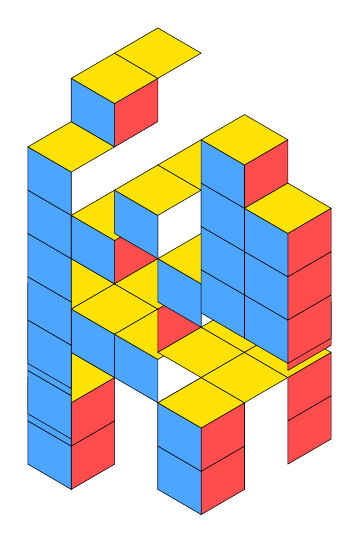
\begin{tikzpicture}[
    x={(0.55cm, -0.32cm)},    % i direction (column, going right)
    y={(-0.55cm, -0.32cm)},   % j direction (row, going into page)
    z={(0cm, 0.55cm)},        % k direction (height, going up)
  ]

  %% Macros for the three face types
  \newcommand{\topface}[3]{% col, row, height
    \fill[yellow!85!orange, draw=black, line width=0.2pt]
      (#1,#2,#3) -- (#1+1,#2,#3) -- (#1+1,#2+1,#3) -- (#1,#2+1,#3) -- cycle;
  }
  \newcommand{\rightface}[3]{% col, row, level (draws right side at col+1)
    \fill[red!70!white, draw=black, line width=0.2pt]
      (#1+1,#2,#3) -- (#1+1,#2+1,#3) -- (#1+1,#2+1,#3+1) -- (#1+1,#2,#3+1) -- cycle;
  }
  \newcommand{\frontface}[3]{% col, row, level (draws front side at row+1)
    \fill[blue!50!cyan!70, draw=black, line width=0.2pt]
      (#1,#2+1,#3) -- (#1+1,#2+1,#3) -- (#1+1,#2+1,#3+1) -- (#1,#2+1,#3+1) -- cycle;
  }

  % Height map: h(col, row)
  % We draw from back to front (large row first, then small row)
  % and from right to left (large col first) for proper occlusion.

  %% --- Row 5 (backmost visible row with data) ---
  % (2,5)=2
  \foreach \l in {0,1} { \rightface{2}{5}{\l} \frontface{2}{5}{\l} }
  \topface{2}{5}{2}

  %% --- Row 4 ---
  % (1,4)=3
  \foreach \l in {0,1,2} { \frontface{1}{4}{\l} }
  \topface{1}{4}{3}
  % (2,4)=3
  \frontface{2}{4}{2}
  \topface{2}{4}{3}
  % (3,4)=3
  \foreach \l in {0,1} { \rightface{3}{4}{\l} }
  \frontface{3}{4}{2}
  \topface{3}{4}{3}
  % (4,4)=2
  \foreach \l in {0,1} { \rightface{4}{4}{\l} }
  \frontface{4}{4}{0} \frontface{4}{4}{1}
  \topface{4}{4}{2}

  %% --- Row 3 ---
  % (0,3)=5
  \foreach \l in {0,1,2,3,4} { \frontface{0}{3}{\l} }
  \topface{0}{3}{5}
  % (1,3)=4
  \rightface{1}{3}{3}
  \frontface{1}{3}{3}
  \topface{1}{3}{4}
  % (2,3)=3
  \rightface{2}{3}{2}
  \topface{2}{3}{3}
  % (3,3)=2
  \topface{3}{3}{2}
  % (4,3)=2
  \topface{4}{3}{2}

  %% --- Row 2 ---
  % (0,2)=6
  \rightface{0}{2}{5}
  \frontface{0}{2}{5}
  \topface{0}{2}{6}
  % (1,2)=4
  \frontface{1}{2}{3}
  \topface{1}{2}{4}
  % (2,2)=3
  \frontface{2}{2}{2}
  \topface{2}{2}{3}
  % (3,2)=2
  \topface{3}{2}{2}
  % (4,2)=2
  \foreach \l in {0,1} { \rightface{4}{2}{\l} }
  \topface{4}{2}{2}

  %% --- Row 1 ---
  % (0,1)=6
  \topface{0}{1}{6}
  % (1,1)=4
  \rightface{1}{1}{3}
  \topface{1}{1}{4}
  % (2,1)=3
  \rightface{2}{1}{2}
  \topface{2}{1}{3}
  % (3,1)=2
  \rightface{3}{1}{1}
  \topface{3}{1}{2}

  %% --- Row 0 (frontmost) ---
  % (1,0)=4
  \rightface{1}{0}{3}
  \foreach \l in {0,1,2,3} { \frontface{1}{0}{\l} }
  \topface{1}{0}{4}
  % (2,0)=3
  \foreach \l in {0,1,2} { \rightface{2}{0}{\l} \frontface{2}{0}{\l} }
  \topface{2}{0}{3}

\end{tikzpicture}
\end{center}

\newpage

%% ============================================================
\section{3D isometric view (cubes stacked on squares)}
%% ============================================================

Each square of the labelled cylindric diagram with label~$k$ is drawn as a stack
of~$k$ unit cubes, viewed from an isometric (axonometric) angle.
The three visible faces of each cube are coloured: yellow (top), blue (left), red (right).
Cubes are drawn back-to-front (painter's algorithm) sorted by depth $c+r$,
so that nearer cubes correctly occlude farther ones.

\bigskip
\begin{center}
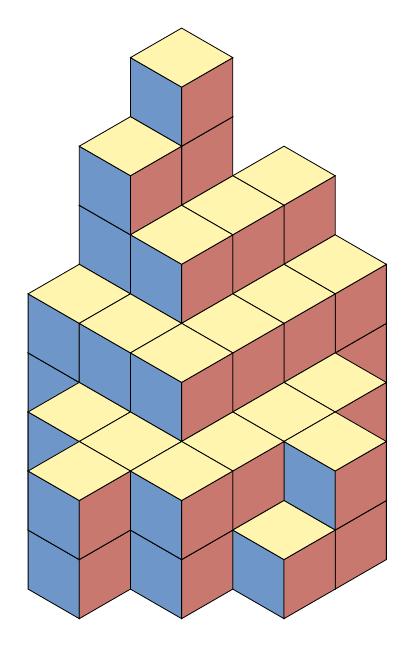
\begin{tikzpicture}[
  % Isometric axes: x = column (lower-right), y = row (lower-left), z = height (up)
  x={(0.65cm, -0.375cm)},
  y={(-0.65cm, -0.375cm)},
  z={(0cm, 0.75cm)}
]

%% Cube face colours
\definecolor{cTop}{RGB}{255,245,175}     % warm yellow
\definecolor{cLeft}{RGB}{110,150,200}    % steel blue
\definecolor{cRight}{RGB}{200,120,110}   % salmon red

%% Macro: draw one unit cube at grid position (c, r, z).
%% Viewer is at (+inf,+inf,+inf), so the THREE VISIBLE faces are:
%%   Top   = z+1 level (horizontal diamond)
%%   Left  = y=r+1 side (left parallelogram on screen)
%%   Right = x=c+1 side (right parallelogram on screen)
%% Draw order: left, right, top (top last covers shared edges cleanly).
\newcommand{\isocube}[3]{%
  % Left face (y=r+1 side, visible from viewer's left)
  \fill[cLeft, draw=black, line width=0.3pt]
    (#1,#2+1,#3) -- (#1+1,#2+1,#3) -- (#1+1,#2+1,#3+1) -- (#1,#2+1,#3+1) -- cycle;
  % Right face (x=c+1 side, visible from viewer's right)
  \fill[cRight, draw=black, line width=0.3pt]
    (#1+1,#2,#3) -- (#1+1,#2+1,#3) -- (#1+1,#2+1,#3+1) -- (#1+1,#2,#3+1) -- cycle;
  % Top face (z+1 level)
  \fill[cTop, draw=black, line width=0.3pt]
    (#1,#2,#3+1) -- (#1+1,#2,#3+1) -- (#1+1,#2+1,#3+1) -- (#1,#2+1,#3+1) -- cycle;
}

%% Draw all cube stacks, sorted by depth c+r (ascending = back to front).
%% Within each depth group, order is irrelevant (no screen overlap).
%% For each position, z iterates 0..h-1 (bottom to top).
%%
%% Data (column, row, height):
%%   Depth 1: (1,0,4), (0,1,6)
%%   Depth 2: (2,0,3), (1,1,4), (0,2,5)
%%   Depth 3: (2,1,3), (1,2,4), (0,3,3)
%%   Depth 4: (3,1,2), (2,2,3), (1,3,3)
%%   Depth 5: (3,2,2), (2,3,3), (1,4,2)
%%   Depth 6: (4,2,2), (3,3,2), (2,4,2)
%%   Depth 7: (4,3,1), (3,4,2), (2,5,2)

\foreach \c/\r/\h in {%
  1/0/4, 0/1/6,%                          depth 1
  2/0/3, 1/1/4, 0/2/5,%                   depth 2
  2/1/3, 1/2/4, 0/3/3,%                   depth 3
  3/1/2, 2/2/3, 1/3/3,%                   depth 4
  3/2/2, 2/3/3, 1/4/2,%                   depth 5
  4/2/2, 3/3/2, 2/4/2,%                   depth 6
  4/3/1, 3/4/2, 2/5/2%                    depth 7
}{%
  \pgfmathtruncatemacro{\maxz}{\h-1}%
  \foreach \z in {0,...,\maxz}{%
    \isocube{\c}{\r}{\z}%
  }%
}

\end{tikzpicture}
\end{center}

\newpage

%% ============================================================
\section{Cylindric repetition (three periods)}
%% ============================================================

The profile $\pi = 10100$ has $n = 2$ ones and $m = 3$ zeros, so each period
the staircase shifts by $(+2, -3)$ in (column, row).
The fundamental domain (Section~7) is shown together with one additional
period to the upper right and one to the lower left, illustrating the cylindric structure.

\bigskip
\begin{center}
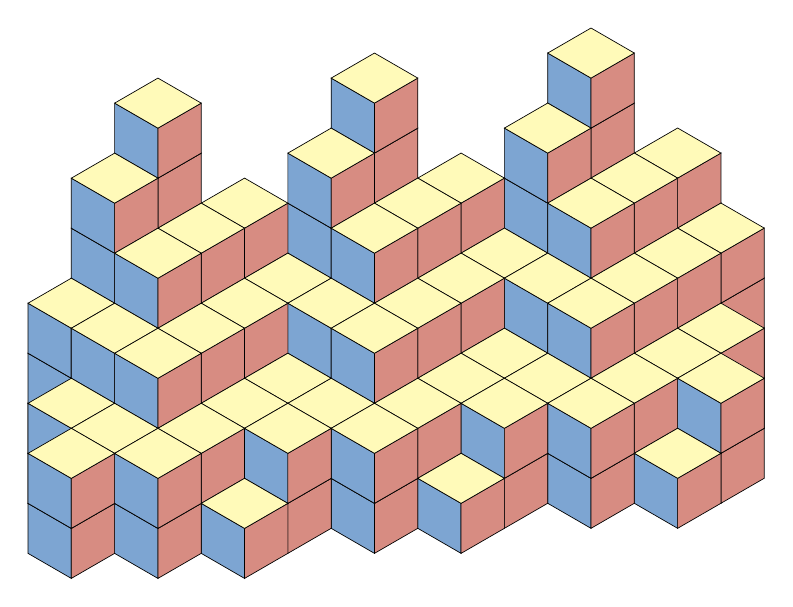
\begin{tikzpicture}[
  x={(0.55cm, -0.318cm)},
  y={(-0.55cm, -0.318cm)},
  z={(0cm, 0.635cm)}
]

\definecolor{cTop}{RGB}{255,250,185}
\definecolor{cLeft}{RGB}{125,165,210}
\definecolor{cRight}{RGB}{215,140,130}

\newcommand{\cube}[3]{%
  \fill[cLeft, draw=black, line width=0.25pt]
    (#1,#2+1,#3) -- (#1+1,#2+1,#3) -- (#1+1,#2+1,#3+1) -- (#1,#2+1,#3+1) -- cycle;
  \fill[cRight, draw=black, line width=0.25pt]
    (#1+1,#2,#3) -- (#1+1,#2+1,#3) -- (#1+1,#2+1,#3+1) -- (#1+1,#2,#3+1) -- cycle;
  \fill[cTop, draw=black, line width=0.25pt]
    (#1,#2,#3+1) -- (#1+1,#2,#3+1) -- (#1+1,#2+1,#3+1) -- (#1,#2+1,#3+1) -- cycle;
}

%% Three periods: Period -1 (shift +2,-3), Period 0 (fundamental), Period +1 (shift -2,+3).
%% Sorted by depth c+r (ascending = back to front).
\foreach \c/\r/\h in {%
  3/{-3}/4, 2/{-2}/6,%                                                         depth 0
  4/{-3}/3, 3/{-2}/4, 2/{-1}/5, 1/0/4, 0/1/6,%                                depth 1
  4/{-2}/3, 3/{-1}/4, 2/0/3, 1/1/4, 0/2/5, {-1}/3/4, {-2}/4/6,%              depth 2
  5/{-2}/2, 4/{-1}/3, 3/0/3, 2/1/3, 1/2/4, 0/3/3, {-1}/4/4, {-2}/5/5,%      depth 3
  5/{-1}/2, 4/0/3, 3/1/2, 2/2/3, 1/3/3, 0/4/3, {-1}/5/4, {-2}/6/3,%         depth 4
  6/{-1}/2, 5/0/2, 4/1/2, 3/2/2, 2/3/3, 1/4/2, 0/5/3, {-1}/6/3,%            depth 5
  6/0/1, 5/1/2, 4/2/2, 3/3/2, 2/4/2, 1/5/2, 0/6/3, {-1}/7/2,%               depth 6
  4/3/1, 3/4/2, 2/5/2, 1/6/2, 0/7/2,%                                         depth 7
  2/6/1, 1/7/2, 0/8/2%                                                         depth 8
}{%
  \pgfmathtruncatemacro{\maxz}{\h-1}%
  \foreach \z in {0,...,\maxz}{%
    \cube{\c}{\r}{\z}%
  }%
}

\end{tikzpicture}
\end{center}

\newpage

%% ============================================================
\section{Profile $\leftrightarrow$ partition bijection}
%% ============================================================

The profile $\pi = 10100$ encodes the base partition $\gamma = (3,2)$
via the boundary path of the Young diagram.
Reading $\pi$ from left to right: $1$ = up step, $0$ = horizontal step.

\bigskip
\begin{center}
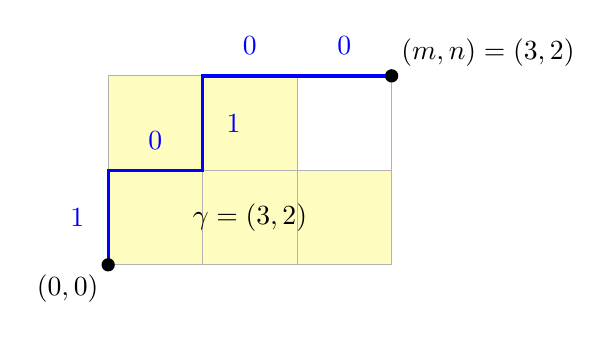
\begin{tikzpicture}[scale=1.2]

  %% Grid
  \draw[gray!40] (0,0) grid (3,2);

  %% Partition cells (shaded)
  % Row 1: 3 cells
  \fill[yellow!25] (0,0) rectangle (3,1);
  % Row 2: 2 cells
  \fill[yellow!25] (0,1) rectangle (2,2);

  %% Redraw grid on top
  \draw[gray!60] (0,0) grid (3,2);

  %% Boundary path (thick)
  \draw[very thick, blue]
    (0,0) -- (0,1) -- (1,1) -- (1,2) -- (2,2) -- (3,2);

  %% Step labels (placed on alternating sides to avoid collision)
  \node[left, blue, font=\bfseries] at (-0.15, 0.5) {$1$};
  \node[above, blue, font=\bfseries] at (0.5, 1.12) {$0$};
  \node[right, blue, font=\bfseries] at (1.15, 1.5) {$1$};
  \node[above, blue, font=\bfseries] at (1.5, 2.12) {$0$};
  \node[above, blue, font=\bfseries] at (2.5, 2.12) {$0$};

  %% Start/end dots
  \fill (0,0) circle (2pt);
  \fill (3,2) circle (2pt);

  %% Labels
  \node[below left] at (0,0) {$(0,0)$};
  \node[above right] at (3,2) {$(m,n) = (3,2)$};

  %% Partition label
  \node at (1.5, 0.5) {$\gamma = (3,2)$};

\end{tikzpicture}
\end{center}

Reading the profile $\pi = \mathbf{1}\,\mathbf{0}\,\mathbf{1}\,\mathbf{0}\,\mathbf{0}$
from left to right traces the staircase boundary from $(0,0)$ to $(m,n)$.
The shaded cells southeast of the path form the partition $\gamma$.

\newpage

%% ============================================================
\section{3D isometric view after peeling ring~3}
%% ============================================================

The cylindric plane partition after peeling ring~3.
All entries $\ge 3$ are reduced: the third ``shell'' of cubes has been removed,
leaving the inner structure exposed.
Positions that had height~$0$ are omitted (no cubes to draw).

\bigskip
\begin{center}
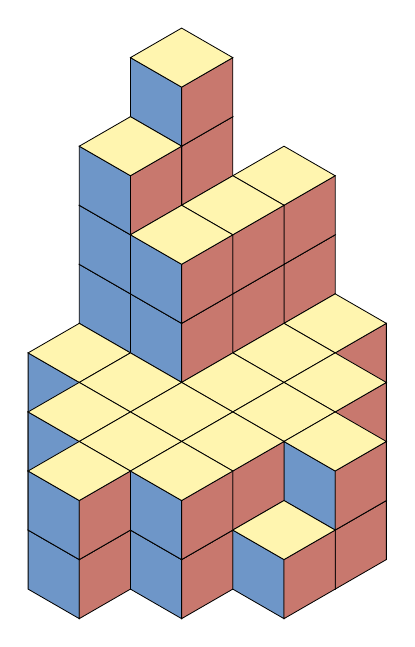
\begin{tikzpicture}[
  x={(0.65cm, -0.375cm)},
  y={(-0.65cm, -0.375cm)},
  z={(0cm, 0.75cm)}
]

\definecolor{cTop}{RGB}{255,245,175}
\definecolor{cLeft}{RGB}{110,150,200}
\definecolor{cRight}{RGB}{200,120,110}

\newcommand{\isocube}[3]{%
  \fill[cLeft, draw=black, line width=0.3pt]
    (#1,#2+1,#3) -- (#1+1,#2+1,#3) -- (#1+1,#2+1,#3+1) -- (#1,#2+1,#3+1) -- cycle;
  \fill[cRight, draw=black, line width=0.3pt]
    (#1+1,#2,#3) -- (#1+1,#2+1,#3) -- (#1+1,#2+1,#3+1) -- (#1+1,#2,#3+1) -- cycle;
  \fill[cTop, draw=black, line width=0.3pt]
    (#1,#2,#3+1) -- (#1+1,#2,#3+1) -- (#1+1,#2+1,#3+1) -- (#1,#2+1,#3+1) -- cycle;
}

%% Height data after peeling ring 3, sorted by depth c+r.
\foreach \c/\r/\h in {%
  1/0/4, 0/1/6,%                          depth 1
  2/0/2, 1/1/4, 0/2/5,%                   depth 2
  2/1/2, 1/2/4, 0/3/2,%                   depth 3
  3/1/2, 2/2/2, 1/3/2,%                   depth 4
  3/2/2, 2/3/2, 1/4/2,%                   depth 5
  4/2/2, 3/3/2, 2/4/2,%                   depth 6
  4/3/1, 3/4/2, 2/5/2%                    depth 7
}{%
  \pgfmathtruncatemacro{\maxz}{\h-1}%
  \foreach \z in {0,...,\maxz}{%
    \isocube{\c}{\r}{\z}%
  }%
}

\end{tikzpicture}
\end{center}

\end{document}
